\documentclass{beamer}

\usepackage[english,ngerman]{babel}
\usepackage[utf8]{inputenc}
\usepackage{microtype}

\usepackage{amsmath, amssymb}

\usepackage{graphicx}
\graphicspath{ {./images/} }

\usepackage{tikz}
\usetikzlibrary{shapes,arrows,positioning}
% Define block styles
\tikzstyle{decision} = [diamond, draw, fill=blue!20, text width=4em, text badly centered, node distance=1.5cm, inner sep=0pt]
\tikzstyle{block} = [rectangle, draw, fill=gray!20, text centered, rounded corners]
\tikzstyle{line} = [draw, -latex']

\usetheme[sectionpage=progressbar]{metropolis}
\beamertemplatenavigationsymbolsempty
\setbeamertemplate{footline}{\insertauthor}

\title{Location Based Recommendations\\Ergebnisse}
\author[H.~Gerdes, J.B.~Latzel, L.~Richardt]{Henrik~Gerdes, Johannes~B.~Latzel, Leon~Richardt}
\institute{Universität Osnabrück}
\date[16.10.2018]{16. Oktober 2018}

\begin{document}
	
	\begin{frame}
		\titlepage
	\end{frame}

	\section{Vorüberlegungen}
	\begin{frame}{Was brauchen wir?}
			\begin{itemize}
				\item \textbf{Datenbank:} Speichert die Events
				\item \textbf{Server:} Entscheidet, welche Events ein Nutzer zu sehen bekommt (\textit{Event Scoring})
				\item \textbf{App:} GUI für den User
				\item \textbf{Client-Server-Interface:} Kommunikation zwischen App und Server
			\end{itemize}
	\end{frame}

	\section{Datenbank}
	\begin{frame}{Datenbank -- Implementation}
		Die Datenbank läuft auf \alert{\texttt{MariaDB}}, einer Open-Source-Alternative zu \texttt{MySQL}. Die Kommunikation zwischen der Datenbank und Java geschieht mit \alert{\texttt{JDBC}} (\textit{Java Database Connectivity}).
		
		\pause
		In der Datenbank gibt es je eine Table für:
		\begin{itemize}
			\item Events
			\item Venues
			\item Tags (\textit{Kategorien, in die die Events eingeordnet werden})
		\end{itemize}
		Außerdem gibt es eine weitere Table, die jedem Event seine Tags zuordnet.
		
	\end{frame}

	\begin{frame}{Datenbank -- Schematischer Aufbau}
		\centering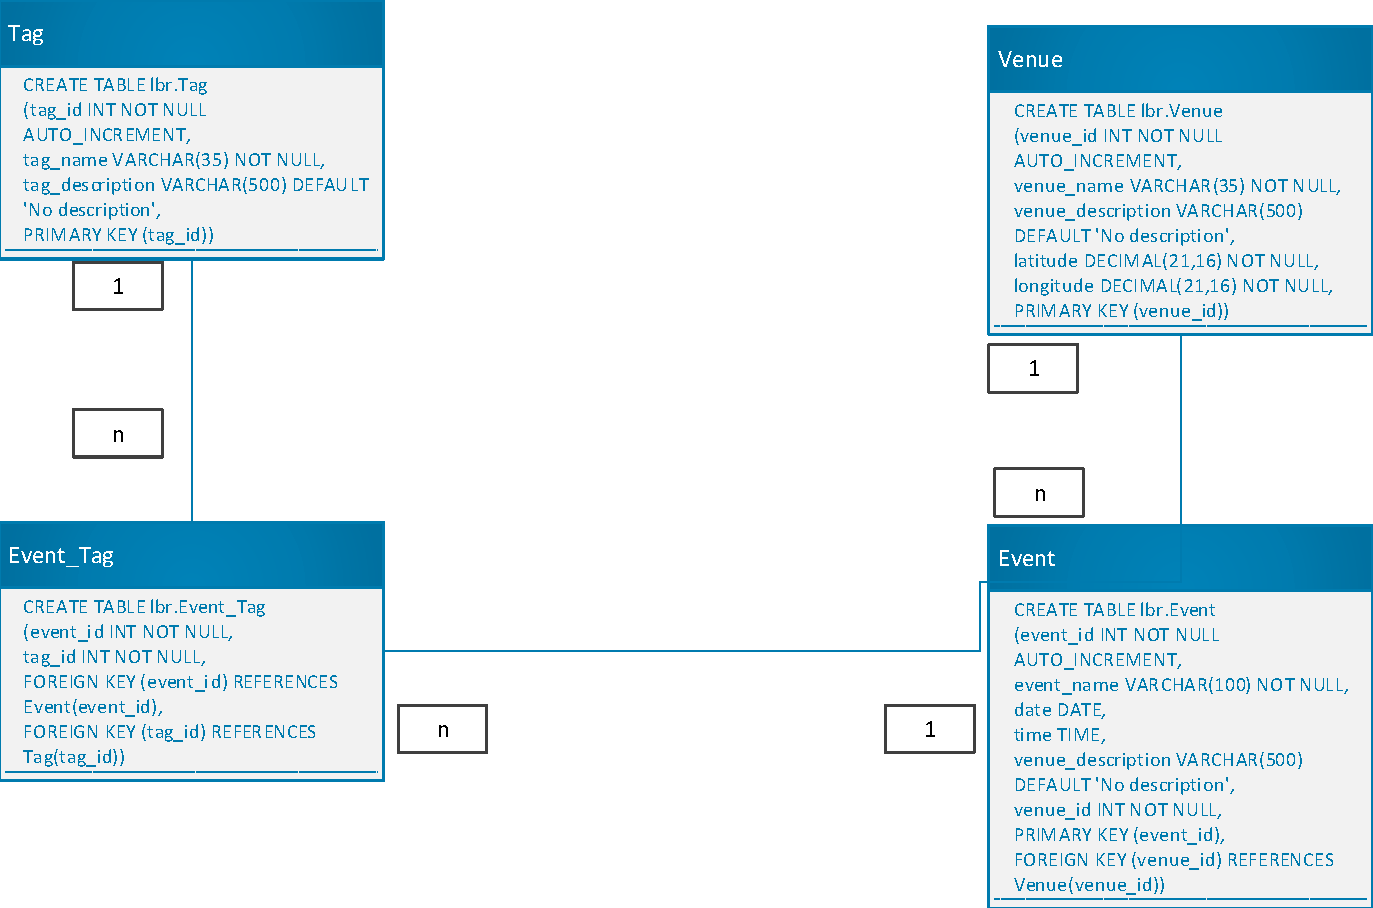
\includegraphics[scale=0.5]{db_scheme}
	\end{frame}

	\section{Server}
	\begin{frame}{Server -- Hardware \& Betriebssystem}
		Als Server wird ein \texttt{Raspberry Pi I B+} mit dem Betriebssystem \texttt{Raspbian} genutzt.
		
		Der Server wartet auf Port \texttt{5445} auf neue Client-Verbindungen und verarbeitet diese. Da ein \alert{Thread-Pool} mit vier Threads genutzt wird, können mehrere Verbindungen gleichzeitig akzeptiert werden.\pause
		
		Kommt es während des Datenbank-Zugriffs zu einer \texttt{SQLException}, so wird automatisch ein \alert{Reconnect} durchgeführt.\pause
		
		Das momentan verwendete \alert{Scoring} ist zufallsbasiert, es ließe sich aber leicht ein anderes Scoring-System integrieren.
	\end{frame}

	\begin{frame}{Server -- Schematischer Ablauf}
		\centering
		\resizebox{!}{\textheight-1.5cm}{%
			\begin{tikzpicture}[node distance = 1cm, auto]
				% Place nodes
				\node (accept) {};
				\node [block, below of=accept] (read) {Lesen aus \texttt{InputStream}};
				\node [decision, below of=read] (class) {Klasse?};
				\node [block, node distance=4cm, left of=class, yshift=-1cm, text width=7em] (readevents) {Events nahe des Nutzers lesen};
				\node [block, right of=filterevents, xshift=2cm, right of=class, yshift=-2cm] (readtags) {alle Tags lesen};
				\node [block, below of=readevents, yshift=-0.3cm] (filterevents) {nach Tags filtern};
				\node [block, below of=filterevents] (scoring) {Scoring};
				\node [block, node distance=4cm, right of=scoring, yshift=-1cm] (createqueryresult) {\texttt{QueryResult} erstellen};
				\node [block, below of=createqueryresult] (writequeryresult) {in \texttt{OutputStream} schreiben};
				\node [block, below of=writequeryresult] (flush) {Flushen und schließen};
				% Draw edges
				\path [line] (accept) -- node [above, yshift=0.2cm] {\footnotesize Eingehende Verbindung} (read);
				\path [line] (read) -- (class);
				\path [line] (class) -| node [above] {\footnotesize\alert<1>{\texttt{LBRQuery}}} (readevents);
				\path [line] (class) -| node [above] {\footnotesize\alert<2>{\texttt{TagQuery}}} (readtags);
				\path [line] (readevents) -- (filterevents);
				\path [line] (filterevents) -- (scoring);
				\path [line] (scoring) |- (createqueryresult);
				\path [line] (readtags) |- (createqueryresult);
				\path [line] (createqueryresult) -- (writequeryresult);
				\path [line] (writequeryresult) -- (flush);
			\end{tikzpicture}
		}
	\end{frame}
	
	\section{Client-Server-Interface}
	\begin{frame}{Client-Server-Interface -- Klassen}
		Folgende Klassen sind besonders wichtig für die Kommunikation zwischen Server und App:
		\begin{itemize}
			\item \texttt{Venue} - Ein Ort, an dem Events stattfinden können
			\item \texttt{Event} - Ein Ereignis, wie z.\,B.\ ein \textit{Konzert} oder ein \textit{Festival}
			\item \texttt{Tag} - Eine Kategorie, wie z.\,B.\ \textit{Tanzen} oder \textit{Live-Musik}
			\item \texttt{Store} - Interface, um Tags und Events zwischenzuspeichern. Mit einem \texttt{StoreListener} kann auf Veränderungen komfortabel reagiert werden.
		\end{itemize}
	\end{frame}
	
	
	\section{App}
	\begin{frame}{App -- Funktionen}
		\begin{itemize}
			\item Der Nutzer landet bei Start auf einem \alert<1>{Splash Screen} und wird erst bei vorhandenen Standort-Berechtigungen weitergeleitet.
			\item Die App führt in regelmäßigen Abständen (15~Minuten) automatisch eine \alert<2>{Aktualisierung} der Events, die in der Nähe stattfinden, durch.
			\item Die aktuelle Position des Users und nahe Events werden auf einer \alert<3>{Karte} angezeigt. Außerdem werden die Events in einer Liste aufgeführt.
			\item Für nahe Events wird ein \alert<4>{Geofence} registriert.
			\item Hält sich der User lange genug innerhalb eines Geofences auf, erhält er eine \alert<5>{Benachrichtigung}.
		\end{itemize}
	\end{frame}

	\section{Herausforderungen}
	\begin{frame}{Herausforderungen bei der Implementation}
		\begin{itemize}
			\item Einarbeitung in Android und in Kotlin
			\item Zuverlässige \alert<1>{Netzwerk-Kommunikation} zwischen App und Server (\textit{Wie kriegen wir die Events vom Server zur App?})
			\item \alert<2>{Eigenheiten} von Android, unter anderem:
				\begin{itemize}
					\item[--] Standortzugriff über den \texttt{FusedLocationProvider}
					\item[--] Regelmäßiges Fetchen von Tags und Events im Hintergrund über \texttt{JobService}
					\item[--] Unzuverlässigkeit der Geofencing-API
				\end{itemize}
			\item Umfangreiche \alert<3>{Frameworks}, die viel Einarbeitung benötigen, wie zum Beispiel:
				\begin{itemize}
					\item[--] Android Job Scheduling
					\item[--] Geofencing
				\end{itemize}
		\end{itemize}
	\end{frame}
	
\end{document}